\documentclass[12pt]{article}
\usepackage{tikz}
\usepackage{collcell}
\usepackage{xcolor}
\usepackage{pgf}

% Define the minimum and maximum values for gradient coloring
\newcommand*{\MinValue}{0}%
\newcommand*{\MaxValue}{100}%

% Apply gradient coloring based on the value
\newcommand{\ApplyGradient}[1]{%
    \pgfmathsetmacro{\PercentColor}{(#1-\MinValue)/(\MaxValue-\MinValue)*100}
    \hspace{-0.33em}\colorbox{yellow!\PercentColor!black}{\textcolor{black}{#1}}
}

\newcolumntype{R}{>{\collectcell\ApplyGradient}c<{\endcollectcell}}
\renewcommand{\arraystretch}{0}
\setlength{\fboxsep}{3mm} % box size
\setlength{\tabcolsep}{0pt}


% PCA reconstructed Idiff delta frequency %

\begin{document}
\begin{table}[ht]
\centering
\caption{PCA reconstructed Idiff delta frequency}
\vspace{10pt} % Add more space here
\begin{tabular}{c *{5}{R}}
\multicolumn{1}{c}{} & \multicolumn{1}{c}{Matched} & \multicolumn{1}{c}{One-Head} & \multicolumn{1}{c}{One-Data} & \multicolumn{1}{c}{Random} & \multicolumn{1}{c}{Sensor} \\
AECno ort & 97.7105 & 41.7010 & 98.9649 & 97.6527 & 34.2682 \\
AECort & 80.0328 & 22.7714 & 80.9933 & 82.3989 & 22.0994 \\
ciPLV & 75.5441 & 71.1222 & 75.2318 & 73.0043 & 68.5206 \\
\end{tabular}

% Color Scale
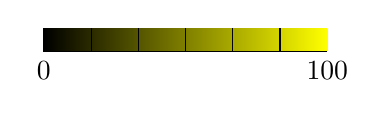
\begin{tikzpicture}[scale=0.6]
    \fill[left color=black, right color=yellow] (0,0) rectangle (6,0.5);
    \draw (0,0) -- (6,0);
    \foreach \x in {0,20,...,100}
        \draw ({\x/20},0) -- ({\x/20},0.5);
    \node[below] at (0,0) {\MinValue};
    \node[below] at (6,0) {\MaxValue};
\end{tikzpicture}
\end{table}

% PCA reconstructed Idiff theta frequency %

\begin{table}[ht]
\centering
\caption{PCA reconstructed Idiff theta frequency}
\vspace{10pt} % Add more space here
\begin{tabular}{c *{5}{R}}
\multicolumn{1}{c}{} & \multicolumn{1}{c}{Matched} & \multicolumn{1}{c}{One-Head} & \multicolumn{1}{c}{One-Data} & \multicolumn{1}{c}{Random} & \multicolumn{1}{c}{Sensor} \\
AECno ort & 98.1096 & 50.1568 & 99.6939 & 98.0548 & 50.8508  \\
AECort &  86.0353 & 30.6471 & 94.1101 & 85.0513 & 38.6159\\
ciPLV & 78.4211 & 71.4845 & 83.3491 & 76.5426 & 74.5152 \\
\end{tabular}

% Color Scale
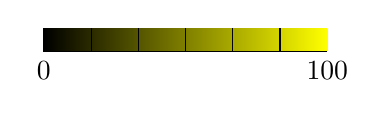
\begin{tikzpicture}[scale=0.6]
    \fill[left color=black, right color=yellow] (0,0) rectangle (6,0.5);
    \draw (0,0) -- (6,0);
    \foreach \x in {0,20,...,100}
        \draw ({\x/20},0) -- ({\x/20},0.5);
    \node[below] at (0,0) {\MinValue};
    \node[below] at (6,0) {\MaxValue};
\end{tikzpicture}
\end{table}

% PCA reconstructed Idiff alpha frequency %

\begin{table}[ht]
\centering
\caption{PCA reconstructed Idiff alpha frequency}
\vspace{10pt} % Add more space here
\begin{tabular}{c *{5}{R}}
\multicolumn{1}{c}{} & \multicolumn{1}{c}{Matched} & \multicolumn{1}{c}{One-Head} & \multicolumn{1}{c}{One-Data} & \multicolumn{1}{c}{Random} & \multicolumn{1}{c}{Sensor} \\
AECno ort & 98.2669 & 53.1695 & 99.0752 & 98.3224 & 49.2962 \\
AECort & 58.7221 & 34.3550 & 92.5666 & 86.6445 & 42.4342 \\
ciPLV & 78.6868 & 72.7385 & 88.5071 & 79.1849 & 76.1705\\
\end{tabular}

% Color Scale
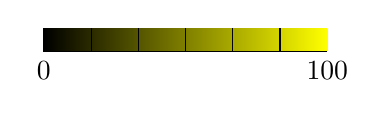
\begin{tikzpicture}[scale=0.6]
    \fill[left color=black, right color=yellow] (0,0) rectangle (6,0.5);
    \draw (0,0) -- (6,0);
    \foreach \x in {0,20,...,100}
        \draw ({\x/20},0) -- ({\x/20},0.5);
    \node[below] at (0,0) {\MinValue};
    \node[below] at (6,0) {\MaxValue};
\end{tikzpicture}
\end{table}


% PCA reconstructed Idiff beta frequency %

\begin{table}[ht]
\centering
\caption{PCA reconstructed Idiff beta frequency}
\vspace{10pt} % Add more space here
\begin{tabular}{c *{5}{R}}
\multicolumn{1}{c}{} & \multicolumn{1}{c}{Matched} & \multicolumn{1}{c}{One-Head} & \multicolumn{1}{c}{One-Data} & \multicolumn{1}{c}{Random} & \multicolumn{1}{c}{Sensor} \\
AECno ort & 99.3391 & 68.8183 & 99.8350 & 99.4464 & 63.7973 \\
AECort & 91.8390 & 49.1177 & 94.4943 & 91.9224 & 48.7780\\
ciPLV & 86.3085 & 79.6876 & 91.3023 & 85.1586 & 79.6668 \\
\end{tabular}

% Color Scale
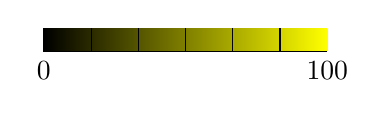
\begin{tikzpicture}[scale=0.6]
    \fill[left color=black, right color=yellow] (0,0) rectangle (6,0.5);
    \draw (0,0) -- (6,0);
    \foreach \x in {0,20,...,100}
        \draw ({\x/20},0) -- ({\x/20},0.5);
    \node[below] at (0,0) {\MinValue};
    \node[below] at (6,0) {\MaxValue};
\end{tikzpicture}
\end{table}


% PCA reconstructed Idiff gamma frequency %

\begin{table}[ht]
\centering
\caption{PCA reconstructed Idiff gamma frequency}
\vspace{10pt} % Add more space here
\begin{tabular}{c *{5}{R}}
\multicolumn{1}{c}{} & \multicolumn{1}{c}{Matched} & \multicolumn{1}{c}{One-Head} & \multicolumn{1}{c}{One-Data} & \multicolumn{1}{c}{Random} & \multicolumn{1}{c}{Sensor} \\
AECno ort & 99.4047 & 54.5748 & 100.0000 & 99.4578 & 60.2089 \\
AECort & 92.4610 & 51.3462 & 98.3418 & 92.6634 & 54.0625\\
ciPLV &  87.0080 & 79.9980 & 95.4418 & 83.4233 & 79.6437\\
\end{tabular}

% Color Scale
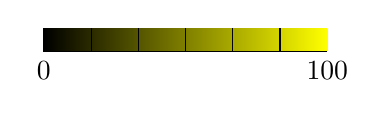
\begin{tikzpicture}[scale=0.6]
    \fill[left color=black, right color=yellow] (0,0) rectangle (6,0.5);
    \draw (0,0) -- (6,0);
    \foreach \x in {0,20,...,100}
        \draw ({\x/20},0) -- ({\x/20},0.5);
    \node[below] at (0,0) {\MinValue};
    \node[below] at (6,0) {\MaxValue};
\end{tikzpicture}
\end{table}
\end{document}




